Dos pequeñas fuentes luminosas, $F_1$ y $F_2$, se encuentran situadas frente a un objeto opaco $AB$, como se observa en la figura de este ejercicio. Recordando la propagación rectilínea de la luz y considerando los puntos señalados en la pantalla, responda:
\begin{enumerate}
    \item ¿Cuáles reciben luz de ambas fuentes?
    \item ¿Cuál sólo la recibe de la fuente $F_1$?
    \item ¿Cuál solamente la capta de la fuente $F_2$?
    \item ¿Cuál no recibe luz de ninguna de las dos fuentes?
\end{enumerate}
\begin{figure}[htb]
  \centering
  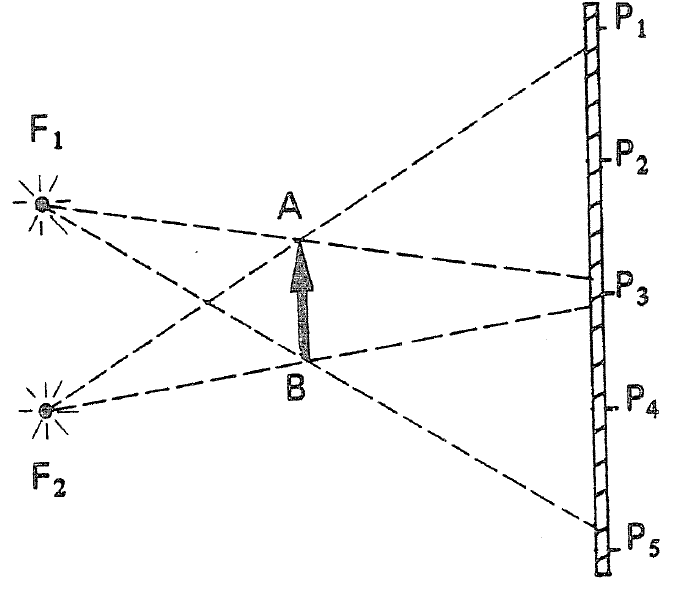
\includegraphics[scale=0.35]{figuras/alvarenga_p615_4.png}
  \caption{Problema 10}
\end{figure}
